\documentclass[10pt,a4paper]{article}
\usepackage[top=3cm,bottom=4cm,left=3.5cm,right=3.5cm]{geometry}
\usepackage{amsmath,amsthm,amsfonts,amssymb,amscd}
\usepackage{fancyhdr,color,comment,graphicx,environ,float,mathtools,mathrsfs,bbm,listings}
\newcommand{\norm}[1]{\left\lVert#1\right\rVert}

% Custom headers
\pagestyle{fancy}
\lhead{ECON - 8050}
\chead{}
\rhead{Tate Mason}
\lfoot{}
\cfoot{\thepage}

\begin{document}

\title{TakeHomeMidterm}
\author{Tate Mason}
\date{}
\maketitle

\section*{Life cycle model}
Consider the problem of a retired person who decumulates a given amount
of wealth $W$. He solves the following problem:

\begin{align*}
    \sum_{t=1}^{T} \beta^t u(c_t) \rightarrow \max_{c,k}
\end{align*}

s.t.\\
total resources of the household:
\begin{align*}
    res_t &= k_t(1 + r) + y_t - x_t\\
    k_1 &= W
\end{align*}

Here $k_t$ is savings, $y_t$ is pension income, and $x_t$ is medical expense shock.
There is a means-tested support program that guarantees each household
consumption at the level $c_{min}$ if his resources are too low. If $res_t > c_{min}$,
then $c_t = res_t - k_{t+1}$, $k_{t+1} \geq 0$. Else, $c_t = c_{min}$ and $k_{t+1} = 0$.

Solve the model using backward induction. Assume CRRA utility function with risk aversion $\sigma$: $u(c_t) = \frac{c_t^{1-\sigma}}{1-\sigma}$. Set $\beta = 0.95$, $r = 0.04$, $\sigma = 3$, $T = 40$, $c_{min} = 0.1$. For income, set $y_t = 1$ for all $t$. For initial wealth set $W = 10$.
Assume $x_t$ can take two values with probability 0.8 and 0.2. Download the
file containing the values for $x_t$ from the course website (xpts40.in). Discretize $k$ using 100 gridpoints, so that $k(1) = 0$ and $k(100) = 100$. Make sure
the grid is more dense around 0. When looking for optimal $k_{t+1}$ do NOT
restrict it to lie on the grid. Make sure you enforce the constraint $k_{t+1} \geq 0$.
(When looking for a maximum you can use Matlab command fminbnd.) To
find value function outside the grid of $k$ use linear interpolation. (When
doing linear interpolation command findnearest can be useful.)

\begin{enumerate}
    \item Solve the model and plot resulting policy functions for $k_{t+1}$ and value
function for ages 10 and 30 fixing $x_t$ at the 1st and 2nd grid.
Organize your graphs as follows: $2 \times 2$ matrix. Left column - savings,
right column - value function. Top row - for age 10, bottom row - age 30.
Each graph should have 2 lines (clearly labeled): fixing $x_t$ at the 1st and
2nd grid (command subplot in Matlab can be useful).

    \item Simulate $\{x_t\}$ for $t = 1 : 40$. Plot savings over the lifecycle using your
policy function.

    \item Increase $c_{min}$ to 0.5 and resolve the model. Plot savings over the life
cycle.

    \item Go back to $c_{min}$ equal to 0.1. Remove medical shock (set $x_t = 0$).
Resolve the model and plot savings over the lifecycle.

    \item Go back to the initial parametrization with medical shock and increase
$\beta$ to 0.99. Resolve the model and plot savings over the lifecycle.

    \item Combine saving profiles from questions 2-5 on the same graph and
compare. Make sure to clearly label each line. Provide economic intuition.
\end{enumerate}

\section*{Solutions}
\subsection*{Part 1}

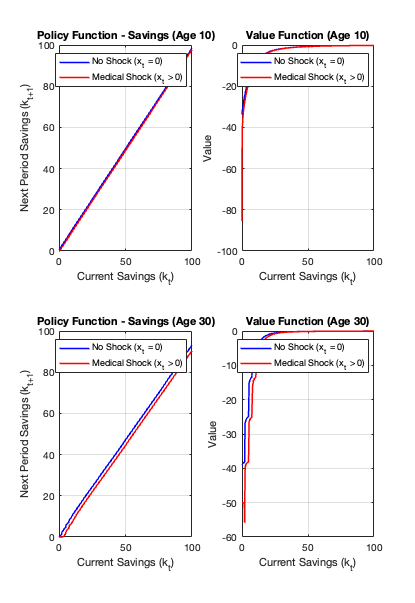
\includegraphics[scale=0.5]{solve_grid.png}

\subsection*{Part 2}

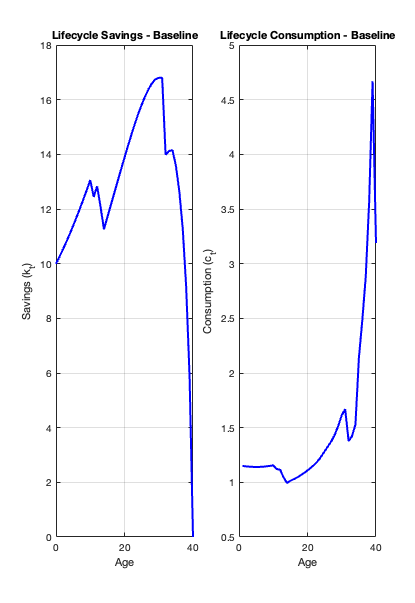
\includegraphics[scale=0.5]{baseline_lifecycle.png}

\subsection*{Part 3}

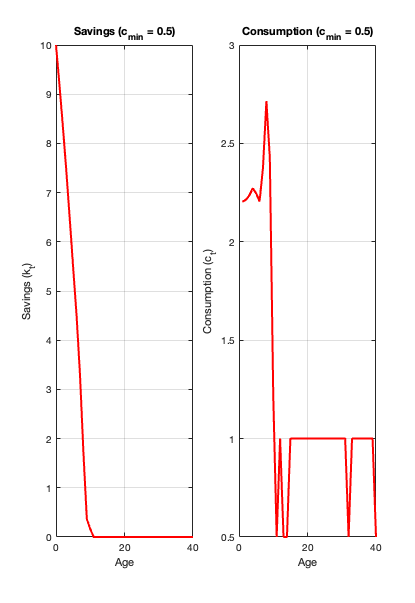
\includegraphics[scale=0.5]{higher_cmin_lifecycle.png}

\subsection*{Part 4}

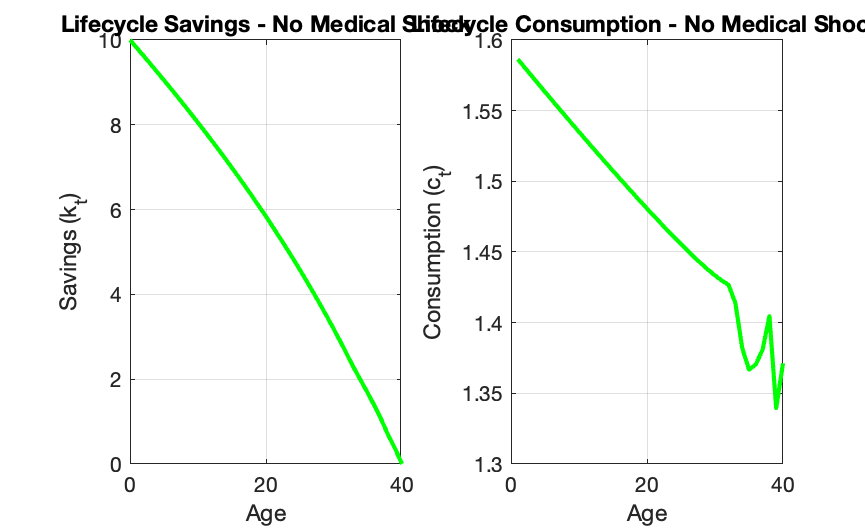
\includegraphics[scale=0.5]{no_shock_lifecycle.png}

\subsection*{Part 5}

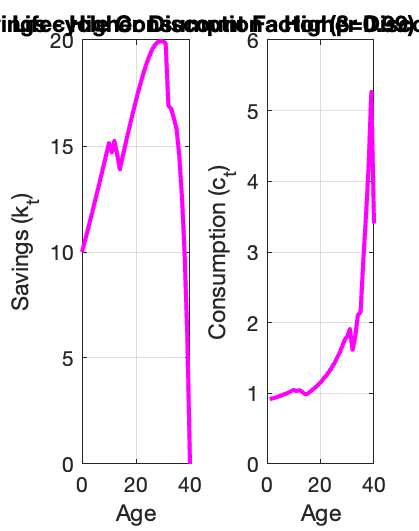
\includegraphics[scale=0.5]{high_beta_lifecycle.png}

\subsection*{Part 6}


As can be seen in the graph above, raising minimum consumption leads to less precautionary saving over the lifetime. As the floor is higher, there is less incentive to hold wealth, instead, agents will consume to meet their needs. In the case of getting rid of the medical shock, there is now incentive to save earlier due to the lack of uncertainty, and a much more linear curve for both savings and consumption. Now, when we raise the discounting rate, we can see an emphasized curve of the one from part 2. This makes sense as, with a higher level of patience (for lack of a better term), they will save more throughout, leading to a steeper decline as period $t=T$ approaches. 


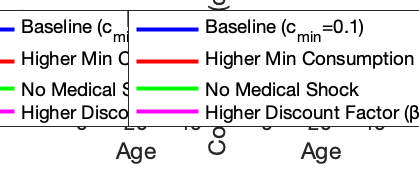
\includegraphics[scale=0.5]{lifecycle_comparison.png}
\end{document}
